\documentclass[a4paper]{article}

\usepackage[utf8]{inputenc}
\usepackage[portuges]{babel}
\usepackage{a4wide}
\usepackage{graphicx}
\usepackage{underscore}
\usepackage{subcaption}
\usepackage{float}

\title{Projeto de Programação Orientada aos Objetos\\Grupo 26 }
\author{Diogo Miguel Alves Rocha (A79751)\and Ricardo Milhazes Veloso (A81919) \and Ricardo Jorge Silva Ferreira (82568)}


\date{\today}
\begin{document}

\maketitle

\begin{figure}[H]
	\centering
	
\includegraphics[width = 420pt,height = 240pt]{nos.png}
	\caption{Elementos do grupo : da esquerda para a direita Ricardo Ferreira, Diogo e Ricardo Veloso}
\end{figure}
\begin{abstract}
 
 Neste relatório faremos a análise ao nosso projeto de Programação Orientada aos Objetos, no qual consiste em criar um programa em Java, chamado JavaFatura com o objetivo de criar um sistema de gestão e dedução de faturas que permita quer a clientes individuais quer a empresas gerir o seu estado fiscal em termos de faturação.

 \end{abstract}

\pagebreak

\tableofcontents

\pagebreak

\section{Introdução}
\label{sec:intro} 

O principal objetivo deste projeto foi desenvolver um programa capaz de registar faturas com a finalidade, de as empresas e os clientes individuais terem acesso às mesmas quer a empresa do montante total de vendas e da dedução a que está sujeita , quer o cliente individual ter acesso ao montante total de gastos e saber qual o montante dedutivel. Para isso será necessário um registo no programa e outras funcionalidades que iremos demonstrar mais à frente neste relatório.


\section{Descrição do Problema}
\label{sec:descricao do problema}
Neste projeto o programa deve ser capaz de gerir o estado fiscal do utilizador para isso deve ser capaz de:

\begin{itemize}
\item Registar um utilizador (Individual ou Empresa);
\item Implementar um login;
\item Criar uma Fatura quer seja uma despesa (C.individual) ou uma venda (C.empresa);
\item Ser possível ao contribuinte individual verificar as faturas emitidas em seu nome , e verificar a respetiva dedução fiscal acumulada;
\item Associar classificação de actividade económica a um documento de despesa;
\item Corrigir a classificação de actividade económica de um documento de despesa;
\item Obter a listagem das facturas de uma determinada empresa, ordenada por data de emissão
ou por valor;
\item Obter por parte das empresas, as listagens das facturas por contribuinte individual num determinado
intervalo de datas;
\item Indicar o total facturado por uma empresa num determinado período;
\item Determinar a relação dos 10 contribuintes que mais gastam em todo o sistema;
\item Determinar as X empresas que mais facturas emitem em todo o sistema e o montante de
deduções fiscais que as despesas registadas (dessas empresas) representam;
\item Gravar o estado da aplicação em ficheiro, para que seja possível retomar mais tarde a execução

\end{itemize}

\pagebreak

\section{Concepção da Solução}
\label{sec:solucao}
A nossa solução foi implementada baseada em diferentes classes , as quais vamos agora especificar:

\begin{itemize}
	\item{Contribuintes}
		\begin{itemize}
			\item{CIndividuais}
			\item{CEmpresas}
		\end{itemize}
	\item{Factura}
	\item{Save_State}
\end{itemize}

\begin{figure}[H]
	\centering
	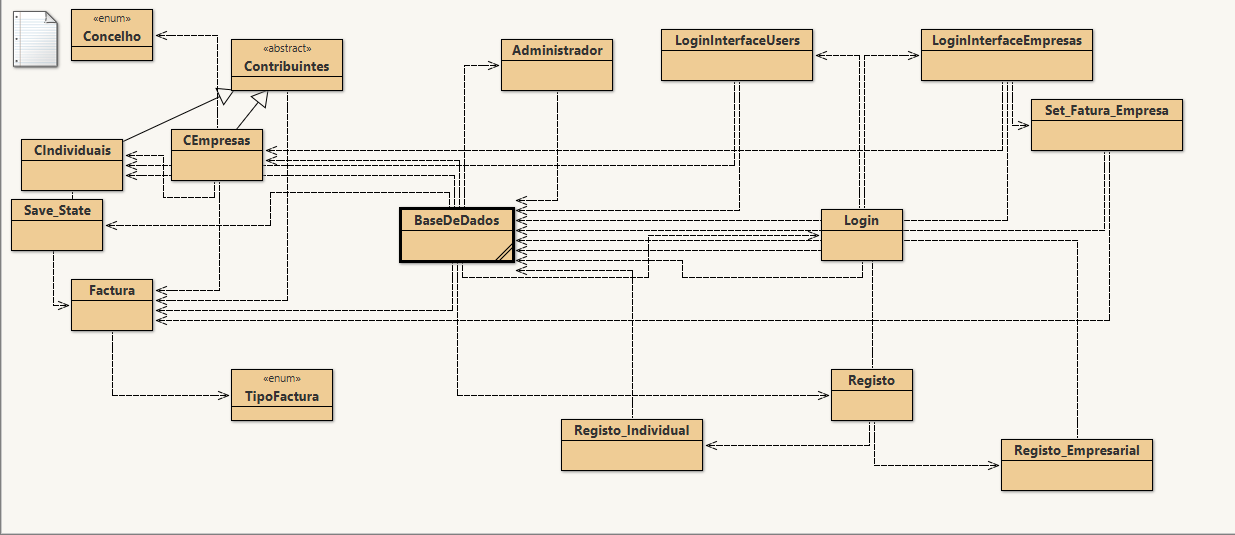
\includegraphics[width = 420pt,height = 240pt]{bluej.png}
	\caption{Bluej}
\end{figure}

\subsection{Contribuintes}
Esta é uma superclasse que define variáveis como : NIF, email,nome,morada,password.

\begin{description}
	\item[CIndividuais] A classe referente aos contribuintes individuais inclui as variáveis definidas na superclasse Contribuintes mas também as variáveis : dependentes, NIFdependentes, coefFiscal, ativEconomicas , despesaTotal, deduzido.

	\item[CEmpresas] A classe referente aos contribuinte Empresas 
	inclui as variáveis definidas na superclasse Contribuintes mas também as variáveis : ativEconomicas , deducoes , concelho , n_faturas , faturado.
\end{description}

\subsection{Factura}
Na classe Factura, classe que nos permite criar uma fatura (apenas disponível para Empresas), são definidas variáveis como : NIFEmitente, designacao , data , NIFCliente , fat, descricao , valorDespesa.

\subsection{Save_State}
Esta é a classe responsável por gravar o estado do programa num determinado momento e permitir a recuperação desse mesmo estado mais tarde. O estado é gravado em ficheiros que se encontram na mesma diretoria do programa.

\subsection{BaseDeDados}
Na implementação deste programa usamos duas HashMap, para guardar informação relativa a Contribuintes Individuais e a Contribuintes Empresas. A nossa escolha baseou-se no uso destas estruturas de dados , principalmente devido aos ganhos em termos de performance em relação a outras estruturas de dados existentes. 

\section{Instruções de utilização}
\label{sec:instrucoes}
Em seguida uma espécie de manual de instruções para a utilização do nosso programa:

	\begin{itemize}
		\item{Criar um utilizador}
			\begin{itemize}
				\item{Contribuinte individual}
				\item{Contribuinte empresa}
			\end{itemize}
		\item{Contribuinte individual}
			\begin{itemize}
				\item{Fazer login no sistema}
				\item{Verificar as depesas emitidas em seu nome e do agregado familiar}
				\item{Corrigir a classificação de atividade económica}
			\end{itemize}
		\item{Contribuinte empresa}
			\begin{itemize}
				\item{Fazer login no sistema}

				\item{Registar uma factura}
				\item{Acesso às faturas por si emitidas}
			\end{itemize}
		\item{Outras funcionalidades}
			\begin{itemize}
				\item{Guardar o estado do programa}
				\item{Determinar os 10 contribuintes que mais gastam em todo o sistema}
			\end{itemize}
	\end{itemize}
\pagebreak
	\subsection{Criar um utilizador}
		\begin{figure}[H]
			\centering
			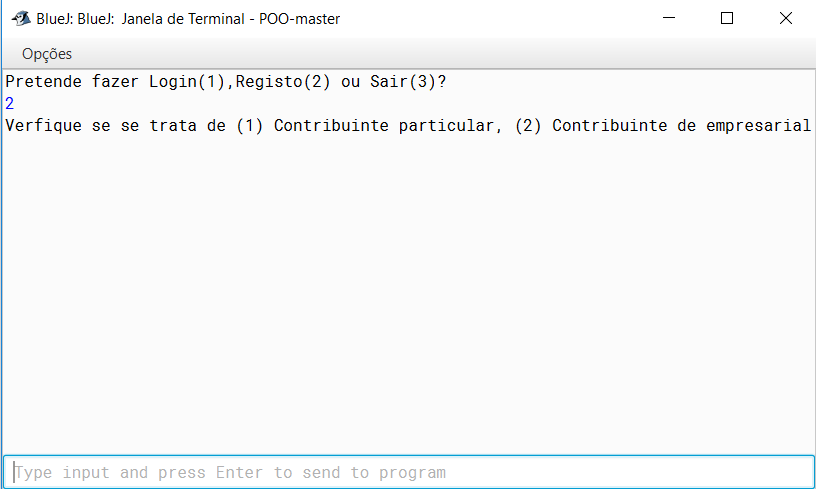
\includegraphics[width = 320pt,height = 140pt]{registo.png}
			\caption{Registo}
		\end{figure}

		\subsubsection{Contribuinte Individual}
			\begin{figure}[H]
				\centering
				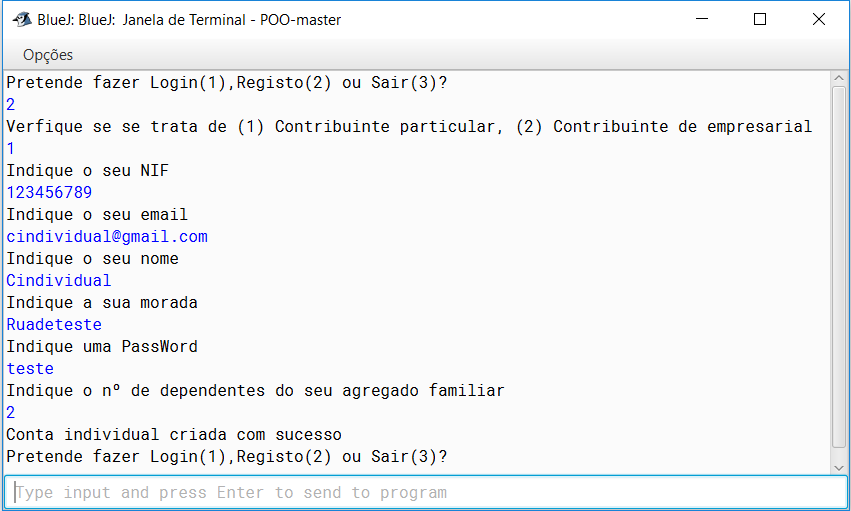
\includegraphics[width = 320pt,height = 140pt]{CI.png}
				\caption{Registo contribuinte individual}
			\end{figure}

		\subsubsection{Contribuinte Empresa}
			\begin{figure}[H]
				\centering
				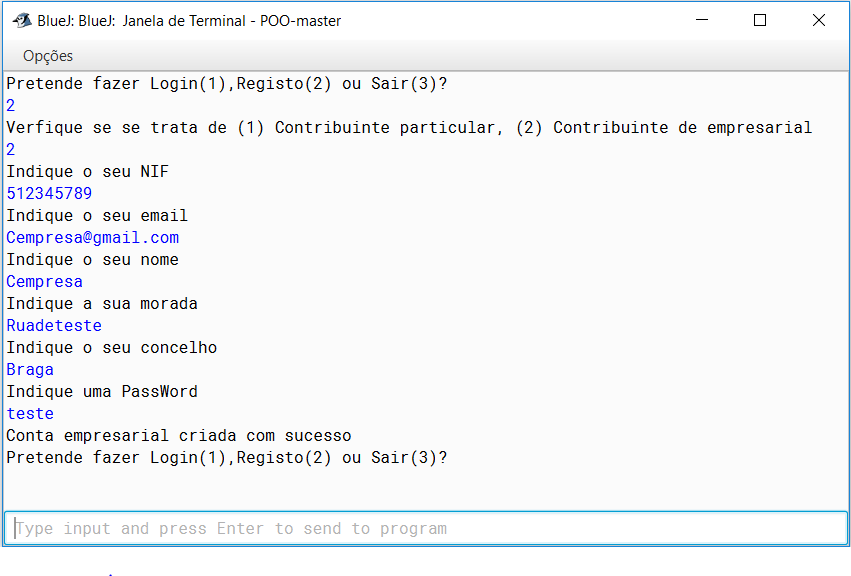
\includegraphics[width = 320pt,height = 140pt]{Ceregisto.png}
				\caption{Registo contribuinte empresa}
			\end{figure}

	\subsection{Contribuinte Individual}

		\subsubsection{Fazer login no sistema}
			\begin{figure}[H]
				\centering
				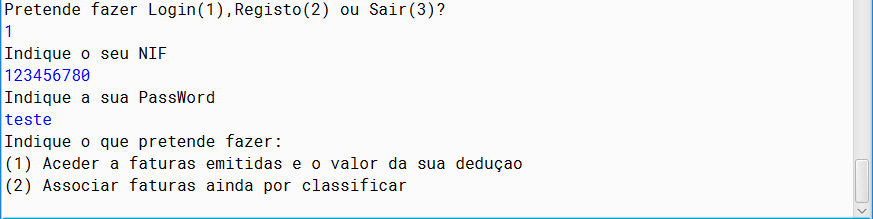
\includegraphics[width = 320pt,height = 140pt]{loginci.png}
				\caption{Login contribuinte individual}
			\end{figure}

		\subsubsection{Verificar as depesas emitidas em seu nome e do agregado familiar}
			\begin{figure}[H]
				\centering
				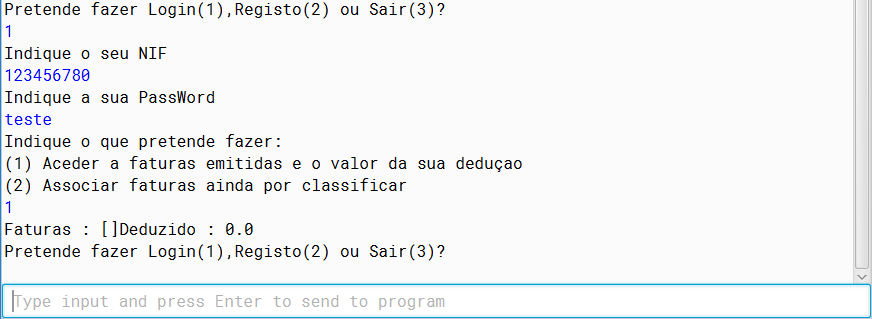
\includegraphics[width = 320pt,height = 140pt]{faturaemitidasci.png}
				\caption{Despesas contribuinte individual}
			\end{figure}

		\subsubsection{Corrigir a classificação de atividade económica}

\pagebreak

	
	\subsection{Contribuinte Empresa}
		\subsubsection{Fazer login no sistema}
			\begin{figure}[H]
				\centering
				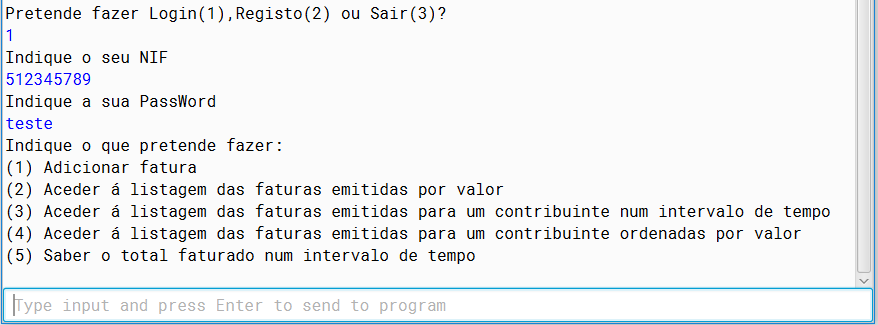
\includegraphics[width = 320pt,height = 140pt]{loginempresa.png}
				\caption{Login contribuinte empresa}
			\end{figure}
		\subsubsection{Registar uma factura}
			\begin{figure}[H]
				\centering
				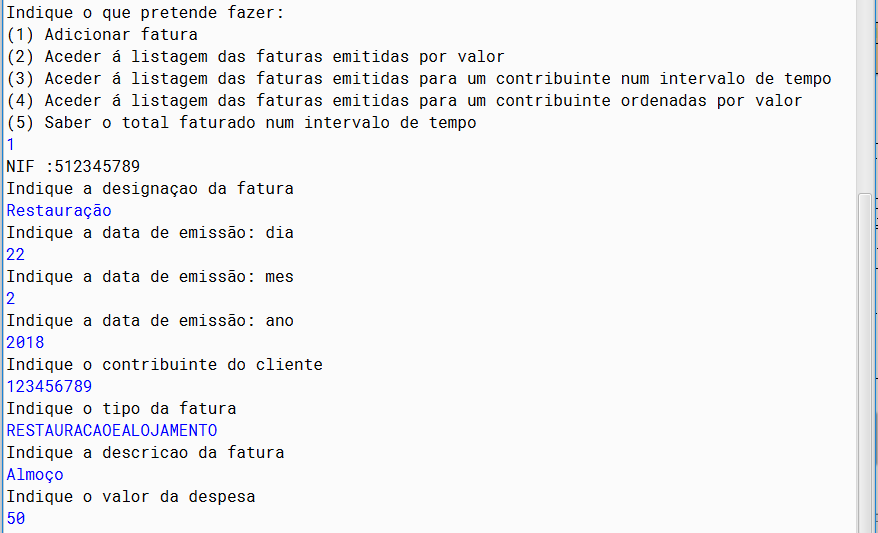
\includegraphics[width = 320pt,height = 240pt]{adicionarfaturaempresa.png}
				\caption{Registar uma factura}
			\end{figure}
		\subsubsection{Acesso às faturas por si emitidas}
		
			\begin{figure}[H]
				\centering
				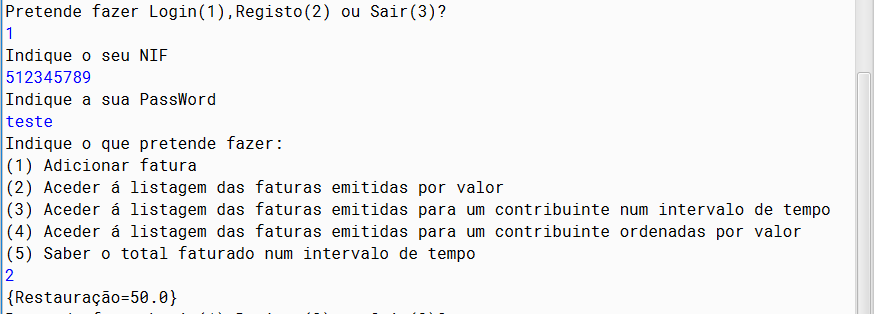
\includegraphics[width = 320pt,height = 240pt]{faturasporvalorEmpresa.png}
				\caption{Faturas ordenadas por valor}
			\end{figure}
				
			\begin{figure}[H]
				\centering
				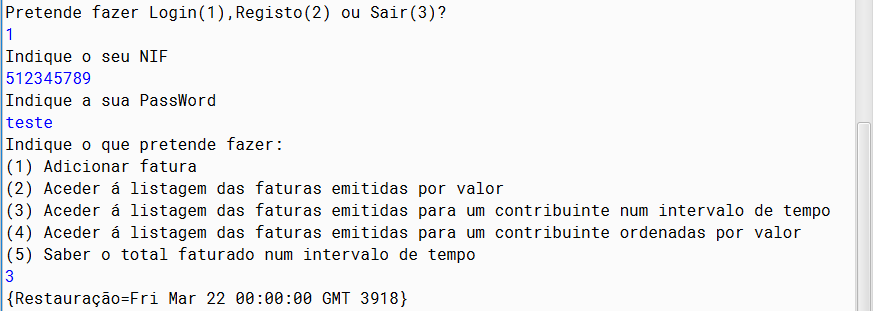
\includegraphics[width = 320pt,height = 240pt]{faturasemitidasporcontibuinte.png}
				\caption{Faturas emitidas por contribuinte num intervalo de tempo}
			\end{figure}
				
			\begin{figure}[H]
				\centering
				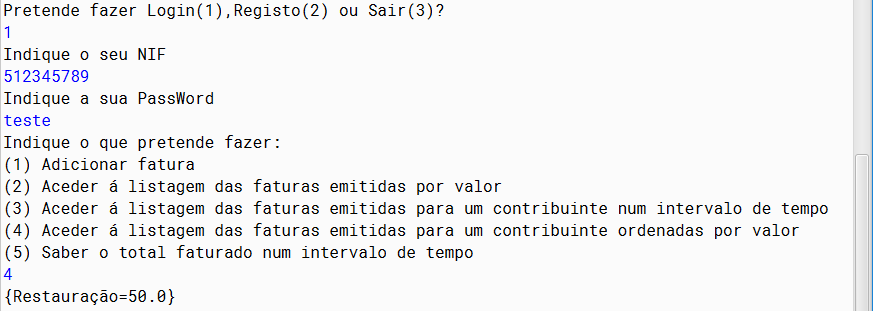
\includegraphics[width = 320pt,height = 240pt]{faturasordenadasporvalor.png}
				\caption{Faturas emitidas por contribuinte ordenadas por valor}
			\end{figure}
				
			\begin{figure}[H]
				\centering
				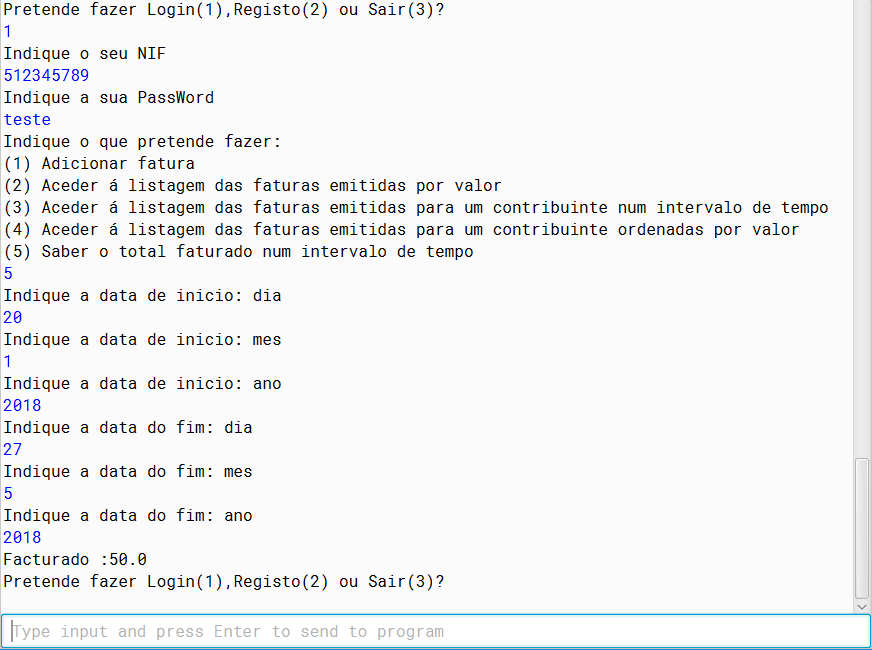
\includegraphics[width = 320pt,height = 240pt]{totalfaturadoempresa.png}
				\caption{Total faturado por uma Empresa num intervalor de tempo}
			\end{figure}
			
	\subsection{Outras funcionalidades}
		\subsubsection{Guardar o estado do programa}
			\begin{figure}[H]
				\centering
				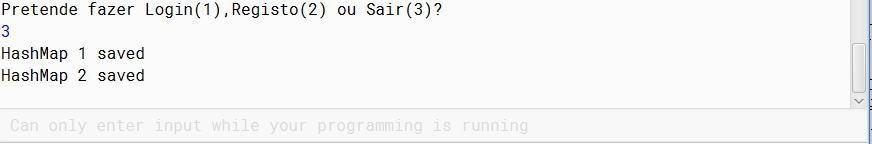
\includegraphics[width = 200pt,height = 130pt]{savestate.png}
				\caption{Guardar o estado do programa}
			\end{figure}
		\subsubsection{Privilegios de admninistrador}
			\begin{figure}[H]
				\centering
				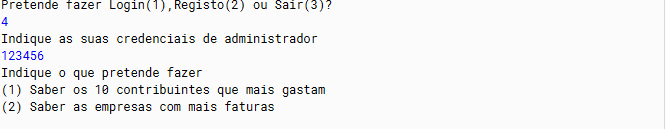
\includegraphics[width = 320pt,height = 200pt]{admin.png}
				\caption{Privilegios de admninistrador}
			\end{figure}

			


			
\section{Conclusão}
\label{sec:conclusao}

Este projeto teve o objetivo de aprofundar os nossos conhecimentos na linguagem de programação JAVA. Permitiu melhorar os nossos recursos tanto em termos do conhecimento da própria linguagem como da aplicação da mesma em problemas da vida real e por consequência uma melhoria na resolução destes e doutros problemas.
Falando especificamente no desenvolvimento do projeto pensamos que foi um trabalho bastante bem conseguido com a resolução de todos os pontos propostos. Em suma foi um projeto bastante positivo com um muito bom funcionamento do grupo conseguindo assim responder a todos os problemas propostos.

\end{document}